\chapter{Finite Markov Chains}\label{C:FiniteMarkovChains}

{\bf NOTE: No materials from this Chapter will be in Probability Theory I exam!}\\[6pt]

{\em This topic is only introduced briefly in Probability Theory I to give concrete instances of dependent sequence of random variables. 
We will revisit these ideas in the sequel. You only need to understand the ideas behind:
\bit
\item Example~\ref{EX:FlippantFreddy} and 
\item Example~\ref{EX:DryWetChain}.
\eit
as done in lectures.}




{
\section{Stochastic Processes}\label{S:StochProc}

\begin{definition}[Stochastic Process]
A collection of RVs  \[
\left(X_{\alpha} \right)_{\alpha \in N} := \left( \  X_{\alpha} : \alpha \in \Az \  \right)
\]
is called a {\bf stochastic process}.  Thus, for every $\alpha \in  \Az$, the index set of the stochastic process, $X_{\alpha}$ is a RV.  If the index set $ \Az  \subset \Zz$ then we have  a {\bf discrete time stochastic process}, typically denoted by 
\[
\left(X_i\right)_{i \in \Zz} := \ldots, X_{-2},X_{-1},X_0, X_1,X_2,\ldots , \  \text{or}
\]
\[
\left( X_i \right)_{i \in \Nz} := X_1,X_2,\ldots , \  \text{or}
\]
\[
\left( X_i \right)_{i \in [n]} := X_1,X_2,\ldots , X_n , \ \text{where, } [n]:= \{1,2,\ldots,n\} \ .
\]
If $\Az \subset \Rz$ then we have a {\bf continuous time stochastic process}, typically denoted by $\{X_t\}_{t \in \Rz}$, etc.  
\end{definition}

Of course the above process is quite general and can allow for arbitrary dependence among the RVs.  
Generally, we cannot produce useful models without making simplifying assumptions. 
The absolutely simplest but extremely useful assumption is that of the {\bf Independent and Identically Distributed or IID Process} or merely {\bf IID Sequence of RVs} when the index set is a subset of $\Nz$. 

This is exactly the sequence of RVs associated with our product experiment $\mathcal{E}^{\otimes \infty} := (\Omega, \mathcal{F}_{\mathcal{X}}, P_{\theta})^{\otimes \infty}$.
    
\begin{definition}[Independent and Identically Distributed (IID) Process]
The finite or infinite sequence of RVs or the stochastic process $X_1, X_2,\ldots$ is said to be independent and identically distributed or IID if :
\begin{itemize}
\item they are an idependently distributed according to \hyperref[D:IndRVs]{Definition \ref*{D:IndRVs}}, and
\item $F(X_1) = F(X_2) = \cdots $, ie.~all the $X_i$'s have the same DF $F(X_1)$.
\end{itemize}
This is perhaps the most elementary class of stochastic processes and we succinctly denote it by
\[
\left(X_i\right)_{i \in [n]} := X_1, X_2,\ldots, X_n \overset{\IID}{\sim} F, \quad \text{or} \quad \left(X_i\right)_{i \in \Nz} := X_1, X_2,\ldots  \overset{\IID}{\sim} F \ .
\]
We sometimes replace the DF $F$ above by the name of the RV.
 \end{definition}
 
\begin{definition}[Independently Distributed]
The sequence of RVs or the stochastic process $\left(X_i\right)_{i \in \Nz} := X_1, X_2,\ldots$ is said to be independently distributed if :
\begin{itemize}
\item $X_1, X_2,\ldots$ is independently distributed according to \hyperref[D:IndRVs]{Definition \ref*{D:IndRVs}}.
\end{itemize}
This is a class of stochastic processes that is more general than the IID class.
\end{definition}

As an example of such a class consider the sequence of RVs that are independent but non-identically distributed with each $X_i \sim \bernoulli(\theta_i)$.

When a stochastic process $\left(X_{\alpha} \right)_{\alpha \in \Az}$ is not independent it is said to be dependent.  
So far we have mostly concerned ourselves with independent processes.  
In this chapter we introduce finite Markov chains and their  simulation methods.
Finit Markov chains are among the simplest stochastic processes with a `first-order' dependence called Markov dependence.

\section{Introduction}\label{S:FiniteMCIntro}
A finite Markov chain is a stochastic process that moves among elements in a finite set $\Xz$ as follows: when at $x \in \Xz$ the next position is chosen at random according to a fixed probability distribution $P(\cdot | x)$.  We define such a process more formally below.

\begin{definition}[Finite Markov Chain]\label{D:TimeHomFiniteMC}
A stochastic sequence, $$\left(X_n\right)_{n \in \Zz_+} := (X_0,X_1,\ldots),$$ is a homogeneous {\bf Markov chain} with {\bf state space} $\Xz$ and {\bf transition matrix} $P:=\left(P(x,y)\right)_{(x,y)\in \Xz^2}$ if for all pair of {\bf states} ${(x,y)\in \Xz^2 := \Xz \times \Xz}$, all integers $t \geq 1$, and all probable historical events $H_{t-1} := \bigcap_{n=0}^{t-1} \{ X_n = x_n \}$ with $\P \left(H_{t-1} \cap \{X_t = x\} \right) > 0$, the following {\bf Markov property} is satisfied: 
\begin{equation}\label{E:FiniteMarkovProperty}
\P\left(X_{t+1} = y | H_{t-1} \cap \{X_t = x\} \right)=\P\left(X_{t+1} = y | X_t = x \right) =: P(x,y) \enspace .
\end{equation}
\end{definition}
The Markov property means that the conditional probability of going to state $y$ at time $t+1$ from state $x$ at current time $t$ is always given by the $(x,y)$-th entry $P(x,y)$ of the transition matrix $P$, no matter what sequence of states $(x_0,x_1,\ldots,x_{t-1})$ preceded the current state $x$.  Thus, the $|\Xz| \times |\Xz|$ matrix $P$ is enough to obtain the state transitions since the $x$-th row of $P$ is the probability distribution $P(x,\cdot) := \left( P(x,y) \right)_{y \in \Xz}$.  For this reason $P$ is called a {\bf stochastic matrix}, i.e.,
\begin{equation}\label{E:StochasticMatrixConds}
P(x,y) \geq 0 \quad \text{for all } (x,y) \in \Xz^2 \qquad \text{and} \quad \sum_{y \in \Xz} P(x,y) = 1 \quad \text{for all } x \in \Xz \enspace .
\end{equation}
Thus, for a Markov chain $\left(X_n\right)_{n \in \Zz_+}$, the distribution of $X_{t+1}$ given $X_0,\ldots,X_t$  depends on $X_t$ alone. Because of this dependence on the previous state, the stochastic sequence, $(X_0,X_1,\ldots)$, are {\it not} independent.  We introduce the most important concepts using a simple example.

\begin{example}[Flippant Freddy]\label{EX:FlippantFreddy}
Freddy the flippant frog lives in an enchanted pond with only two lily pads, {\em rollopia} and {\em flipopia}.  A wizard gave a  die and a silver coin to help flippant Freddy decide where to jump next.  Freddy left the die on rollopia and the coin on flipopia.  When Freddy got restless in rollopia he would roll the die and if the die landed odd he would leave the die behind and jump to flipopia, otherwise he would stay put.  When Freddy got restless in flipopia he would flip the coin and if it landed Heads he would leave the coin behind and jump to rollopia, otherwise he would stay put.

Let the state space $\Xz=\{r,f\}$, and let $(X_0, X_1,\ldots)$ be the sequence of lily pads occupied by Freddy after his restless moments.  Say the die on rollopia $r$ has probability $p$ of turning up odd and the coin on flipopia $f$ has probability $q$ of turning up heads.  We can visualise the rules of Freddy's jumps by the following {\bf transition diagram}:
\begin{figure}[htpb]
\caption{Transition Diagram of Flippant Freddy's Jumps.\label{F:FlippantFreddyTransDiag}}
\centering   \makebox{\includegraphics[width=6.5in]{figures/FlippantFreddyTransDiag}}
\end{figure}

Then Freddy's sequence of jumps $(X_0, X_1,\ldots)$ is a Markov chain on $\Xz$ with transition matrix:
\begin{equation}\label{E:FlippantFreddyP}
P 
= \bordermatrix{~ & r & f \cr 
r & P(r,r) & P(r,f)\cr 
f & P(f,r) & P(f,f) }
= \bordermatrix{~ & r & f \cr 
r & 1-p & p \cr
f & q & 1-q } \enspace .
\end{equation}
Suppose we first see Freddy in rollopia, i.e., $X_0=r$.  When he gets restless for the first time we know from the first row of $P$ that he will leave to flippopia with probability $p$ and stay with probability $1-p$, i.e.,
\begin{equation}\label{E:Freddy1Step}
\P(X_1=f | X_0=r) = p, \quad \P(X_1=r | X_0=r) = 1-p \enspace .
\end{equation}
What happens when he is restless for the second time?  By considering the two possibilities for $X_1$, Definition of conditional probability and the Markov property, we see that,
\begin{eqnarray}
\P(X_2 = f | X_0 = r) 
&=& \P(X_2=f, X_1=f | X_0=r) + \P(X_2=f, X_1=r | X_0=r) \notag \\
&=& \frac{\P(X_2=f, X_1=f , X_0=r)}{\P(X_0=r)} + \frac{\P(X_2=f, X_1=r , X_0=r)}{\P(X_0=r)} \notag \\
&=& \P(X_2=f | X_1=f , X_0=r)\frac{\P(X_1=f , X_0=r)}{\P(X_0=r)} \notag \\
&& \qquad + \P(X_2=f | X_1=r , X_0=r) \frac{\P(X_1=r , X_0=r)}{\P(X_0=r)} \notag \\
%&=& \frac{\P(X_2=f | X_1=f , X_0=r)\P(X_1=f | X_0=r)\P(X_0=r)}{\P(X_0=r)} \\
%&& \qquad + \frac{\P(X_2=f | X_1=r , X_0=r) \P(X_1=r | X_0=r)\P(X_0=r)}{\P(X_0=r)} \\
&=&{\P(X_2=f | X_1=f , X_0=r)\P(X_1=f | X_0=r)} \notag \\
&& \qquad +{\P(X_2=f | X_1=r , X_0=r) \P(X_1=r | X_0=r)} \notag \\
&=& \P(X_2=f | X_1=f) \P(X_1=f | X_0=r) \notag \\
&& \qquad+ \P(X_2=f | X_1=r) \P(X_1=r | X_0=r) \notag \\
&=& P(f,f) P(r,f) + P(r,f) P(r,r) \notag \\
&=& (1-q) p + p (1-p) \label{E:Freddy2Stepa}
\end{eqnarray}
Similarly, 
\begin{equation} \label{E:Freddy2Stepb}
\P(X_2=r | X_0 =r) = P(f,r) P(r,f) + P(r,r) P(r,r) = q p + (1-p)(1-p)
\end{equation}
Instead of elaborate computations of the probabilities of being in a given state after Freddy's $t$-th restless moment, we can store the state probabilities at time $t$ in a row vector:
\[
\mu_t := \left(  \P(X_t = r | X_0 = r), \P(X_t=f | X_0=r) \right) \enspace ,
\]
Now, we can conveniently represent Freddy starting in rollopia by the {\bf initial distribution} $\mu_0 = (1,0)$ and obtain the 1-step {\bf state probability vector} in \eqref{E:Freddy1Step} from $\mu_1 = \mu_0 P$ and the 2-step state probabilities in \eqref{E:Freddy2Stepa} and \eqref{E:Freddy2Stepb} by $\mu_2 = \mu_1 P = \mu_0 P P = \mu_0 P^2$.  In general, multiplying $\mu_t$, the state probability vector at time $t$, by the transition matrix $P$ on the right updates the state probabilities by another step:
\[
\mu_{t} = \mu_{t-1} P \qquad \text{for all } t \geq 1 \enspace .
\]
And for any initial distribution $\mu_0$,
\[
\mu_{t} = \mu_0 P^t  \qquad \text{for all } t \geq 0 \enspace .
\]
This can be easily implemented in \Matlab as follows:
%\begin{VrbM}
%>> p=0.5; q=0.5; P = [1-p p; q 1-q] % assume a fair coin and a fair die
%P =
%    0.5000    0.5000
%    0.5000    0.5000
%
%>> mu0 = [1, 0] % inital state vector since Freddy started in rollopia
%mu0 =     1     0
%
%>> mu0*P^0    % intial state distribution at t=0 is just mu0
%ans =     1     0
%
%>> mu0*P^1    % state distribution at t=1
%ans =    0.5000    0.5000
%
%>> mu0*P^2    % state distribution at t=2
%ans =    0.5000    0.5000
%\end{VrbM}
%Thus for a fair coin and die we get equal probabilities of being in the two states right after the first jump.  Let us see what happens for an unfair coin and die:
\begin{VrbM}
>> p=0.85; q=0.35; P = [1-p p; q 1-q] % assume an unfair coin and an unfair die
P =
    0.1500    0.8500
    0.3500    0.6500
>> mu0 = [1, 0] % inital state vector since Freddy started in rollopia
mu0 =     1     0
>> mu0*P^0    % intial state distribution at t=0 is just mu0
ans =     1     0
>> mu0*P^1    % state distribution at t=1
ans =    0.1500    0.8500
>> mu0*P^2    % state distribution at t=2
ans =    0.3200    0.6800
>> mu0*P^3    % state distribution at t=3
ans =    0.2860    0.7140
\end{VrbM}
Now, let us compute and look at the probability of being in rollopia after having started there for three values of $p$ and $q$ according to the following script: 
\VrbMf[label=FlippantFreddyRollopiaProbs.m]{scripts/FlippantFreddyRollopiaProbs.m}

\begin{figure}[htpb]
\caption{The probability of being back in rollopia in $t$ time steps after having started there under transition matrix $P$ with (i) $p=q=0.5$ (blue line with asterisks), (ii) $p=0.85$, $q=0.35$ (black line with dots) and (iii) $p=0.15$, $q=0.95$ (red line with pluses).\label{F:FlippantFreddyRollopiaProbs}}
\centering   \makebox{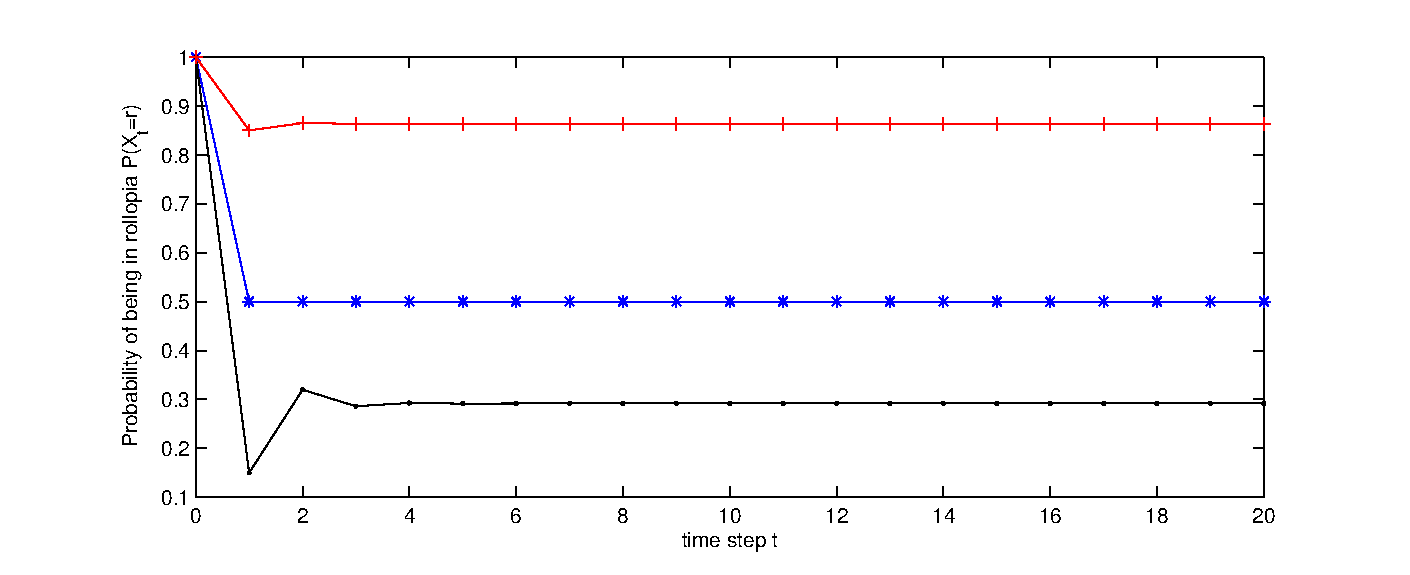
\includegraphics[width=6.5in]{figures/FlippantFreddyRollopiaProbs}}
\end{figure}

It is evident from \hyperref[F:FlippantFreddyRollopiaProbs]{Figure~\ref*{F:FlippantFreddyRollopiaProbs}} that as $t \to \infty$, $\mu_t$ approaches a distribution, say $\pi$, that depends on $p$ and $q$ in $P$.  Such a limit distribution is called the {\bf stationary distribution} and must satisfy the fixed point condition:
\[
\pi P = \pi \enspace ,
\]
that gives the solution:
\[
\pi(r) = \frac{q}{p+q}, \qquad \pi(f) = \frac{p}{p+q} \enspace .
\]
In \hyperref[F:FlippantFreddyRollopiaProbs]{Figure~\ref*{F:FlippantFreddyRollopiaProbs}} we see that $\P(X_t=r)$ approaches $\pi(r) = \frac{q}{p+q}$ for the three cases of $p$ and $q$:
\begin{align*}
\text{(i)}& \ p=0.50, q=0.50, & \P(X_t=r) & \to \pi(r) = \frac{q}{p+q} =  \frac{0.50}{0.50+0.50} = 0.5000,\\
\text{(ii)}& \  p=0.85, q=0.35, & \P(X_t=r) & \to \pi(r) = \frac{q}{p+q} =  \frac{0.35}{0.85+0.35} = 0.2917, \\
\text{(iii)}& \ p=0.15, q=0.95, & \P(X_t=r) & \to \pi(r) = \frac{q}{p+q} = \frac{0.95}{0.15+0.95} = 0.8636.
\end{align*}
\end{example}

Now let us generalise the lessons learned from \hyperref[EX:FlippantFreddy]{Example~\ref*{EX:FlippantFreddy}}.

\begin{prop}\label{P:FiniteMCProbsAtTimet}
For a finite Markov chain $\left(X_t\right)_{t \in \Zz_+}$ with state space $\Xz=\{s_1,s_2,\ldots,s_k\}$, initial distribution $$\mu_0 := \left( \mu_0(s_1), \mu_0(s_2), \ldots, \mu_0(s_k) \right),$$ where $\mu_0(s_i) = \P(X_0=s_i)$, and transition matrix $$P := \left(P(s_i,s_j)\right)_{(s_i,s_j)\in \Xz^2},$$ we have for any $t \in \Zz_+$ that the distribution at time $t$ given by:
$$\mu_t := \left( \mu_t(s_1), \mu_t(s_2), \ldots, \mu_t(s_k) \right),$$
where $\mu_t(s_i) = \P(X_t=s_i)$, satisfies:
\begin{equation}\label{E:mutismu0Pt}
\mu_t = \mu_0 P^t \enspace .
\end{equation}
\begin{proof}
We will prove this by induction on $\Z_+:=\{0,1,2,\ldots\}$.  First consider the case when $t=0$.  Since $P^0$ is the identity matrix $I$, we get the desired equality:
\[
\mu_0 P^0 = \mu_0 I = \mu_0 \enspace .
\]
Next consider the case when $t=1$.  We get for each $j \in \{1,2,\ldots,k\}$, that
\begin{align*}
\mu_1(s_j) &= \P(X_1 = s_j) = \sum_{i=1}^k \P(X_1=s_j,X_0=s_i)\\
&= \sum_{i=1}^k \P(X_1=s_j | X_0=s_i) \P(X_0=s_i) \\
&= \sum_{i=1}^k P(s_i,s_j) \mu_0(s_i)\\
&= (\mu_0 P)(s_j), \quad \text{the $j$-th entry of the row vector $(\mu_0 P)$} \enspace .
\end{align*}
Hence, $\mu_1=\mu_0 P$.  Now, we will fix $m$ and suppose that \eqref{E:mutismu0Pt} holds for $t=m$ and prove that \eqref{E:mutismu0Pt} also holds for $t=m+1$.  
For each $j \in \{1,2,\ldots,k\}$, we get
\begin{align*}
\mu_{m+1}(s_j) &= \P(X_{m+1} = s_j) = \sum_{i=1}^k \P(X_{m+1}=s_j,X_m=s_i)\\
&= \sum_{i=1}^k \P(X_{m+1}=s_j | X_m=s_i) \P(X_m=s_i) \\
&= \sum_{i=1}^k P(s_i,s_j) \mu_m(s_i)\\
&= (\mu_m P)(s_j), \quad \text{the $j$-th entry of the row vector $(\mu_m P)$} \enspace .
\end{align*}
Hence, $\mu_{m+1}=\mu_m P$.  But $\mu_{m}=\mu_0 P^m$ by the induction hypothesis, and therefore:
\[
\mu_{m+1} = \mu_m P = \mu_0 P^m P = \mu_0 P^{m+1} \enspace .
\]
Thus by the principle of mathematical induction we have proved the proposition.
\end{proof}
\end{prop}
Thus, multiplying a row vector $\mu_0$ by $P^t$ on the right takes you from current distribution over the state space to the distribution in $t$ steps of the chain.  

Since we will be interested in Markov chains on $\Xz =\{s_1,s_2,\ldots,s_k\}$ with the same transition matrix $P$ but different initial distributions, we introduce $\P_{\mu}$ and $\E_{\mu}$ for probabilities and expectations  given that the initial distribution is $\mu$, respectively.  When the initial distribution is concentrated at a single initial state $x$ given by:
$$\BB{1}_{\{x\}}(y) := \begin{cases} 1 & \text{if } y=x\\ 0 & \text{if } y \neq x \end{cases}$$ 
we represent it by $e_x$, the $1 \times k$ ortho-normal basis row vector with a $1$ in the $x$-th entry and a $0$ elsewhere.  
We simply write $\P_x$ for $\P_{\BB{1}_{\{x\}}}$ or $\P_{e_x}$ and $\E_x$ for $\E_{\BB{1}_{\{x\}}}$ or $\E_{e_x}$.  Thus, \hyperref[P:FiniteMCProbsAtTimet]{Proposition~\ref*{P:FiniteMCProbsAtTimet}} along with our new notations means that:
\[
\P_x (X_t = y)  = (e_x P^t)(y) = P^t(x,y) \enspace .
\]
In words, the probability of going to $y$ from $x$ in $t$ steps is given by the $(x,y)$-th entry of $P^t$, the {\bf $t$-step transition matrix}.  We refer to the $x$-th row and the $x$-th column of $P$ by $P(x,\cdot)$ and $P(\cdot,x)$, respectively.

Let the function $f(x): \Xz\to \Rz$ be represented by the column vector $f := (f(s_1),f(s_2),\ldots,f(s_k)) \in \Rz^{k \times 1}$.  Then the $x$-th entry of $P^t f$ is:
\[
P^t f(x) = \sum_{y} P^t(x,y) f(y) = \sum_{y} f(y) \P_x (X_t = y) = \E_x (f(X_t)) \enspace .
\] 
This is the expected value of $f$ under the distribution of states in $t$ steps given that we start at state $x$.  
Thus multiplying a column vector $f$ by $P^t$ from the left takes you from a function on the state space to its expected value in $t$ steps of the chain. 

%Let us look at some more examples of Markov chains.
\begin{example}[Dry-Wet Christchurch Weather]\label{EX:DryWetChain}
Consider a toy weather model for dry or wet days in Christchurch using a Markov chain with state space $\{d,w\}$.  Let the transition diagram in \hyperref[F:DryWetTransDiag]{Figure~\ref*{F:DryWetTransDiag}} give the transition matrix $P$ for our dry-wet Markov chain.  
\begin{figure}[htpb]
\caption{Transition Diagram of Dry and Wet Days in Christchurch.\label{F:DryWetTransDiag}}
\centering   \makebox{\includegraphics[width=3.5in]{figures/DryWetTransDiag}}
\end{figure}
Using \eqref{E:mutismu0Pt} we can find that the probability of being dry on the day after tomorrow is $0.625$ given that it is wet today as follows:
\begin{VrbM}
>> P=[0.75 0.25; 0.5 0.5] % Transition Probability Matrix
P =
    0.7500    0.2500
    0.5000    0.5000
>> mu0=[0 1] % it is wet today gives the initial distribution
mu0 =     0     1
>> mu0 * P^2 % the distribution in 2 days from today
ans =    0.6250    0.3750
\end{VrbM}
Suppose you sell \$100 of lemonade at a road-side stand on a hot day but only \$50 on a cold day.  Then we can compute your expected sales tomorrow if today is dry as follows:
\begin{VrbM}
>> P=[0.75 0.25; 0.5 0.5] % Transition Probability Matrix
P =
    0.7500    0.2500
    0.5000    0.5000
>> f = [100; 50] % sales of lemonade in dollars on a dry and wet day
f =
   100
    50
>> P*f % expected sales tomorrow
ans =
   87.5000
   75.0000 
>> mu0 = [1 0] % today is dry
mu0 =     1     0
>> mu0*P*f % expected sales tomorrow if today is dry
ans =   87.5000
\end{VrbM}
\end{example}

\begin{exercise}[Freddy discovers a gold coin]\label{EXR:FreddyGoldCoin}
Flippant Freddy of \hyperref[EX:FlippantFreddy]{Example~\ref*{EX:FlippantFreddy}} found a gold coin at the bottom of the pond.  Since this discovery he  jumps around differently in the enchanted pond.  He can be found now in one of three states: flipopia, rollopia and hydropia (when he dives into the pond). His state space is $\Xz=\{r,f,h\}$ now and his transition mechanism is as follows: If he rolls an odd number with his fair die in rollopia he will jump to flipopia but if he rolls an even number then he will stay in rollopia only if the outcome is $2$ otherwise he will dive into hydropia.  If the fair gold coin toss at the bottom of hydropia is Heads then Freddy will swim to flipopia otherwise he will remain in hydropia. Finally, if he is in flipopia he will remain there if the silver coin lands Heads otherwise he will jump to rollopia.

Make a Markov chain model of the new jumping mechanism adopted by Freddy.  Draw the transition diagram, produce the transition matrix $P$ and compute using \Matlab the probability that Freddy will be in hydropia after one, two, three, four and five jumps given that he starts in hydropia.
\end{exercise}

\begin{exercise}\label{Exr:NonMarkovProjection1}
Let $(X_t)_{t\in\Zz_+}$ be a Markov chain with state space $\{a,b,c\}$, initial distribution $\mu_0=(1/3,1/3,1/3)$ and transition matrix 
$$P = 
\bordermatrix{~ & a & b & c \cr
a & 0 & 1 & 0\cr
b & 0 & 0 & 1\cr
c & 1 & 0 & 0} \enspace .
$$
For each $t$, define $Y_t = \BB{1}_{\{b,c\}}(X_t)$.  Show that $(Y_t)_{t\in\Zz_+}$ is not a Markov chain.
\end{exercise}

\begin{exercise}\label{Exr:RegularSampledChainIsMarkov}
Let $(X_t)_{t\in\Zz_+}$ be a (homogeneous) Markov chain on $\Xz=\{s_1,s_2,\ldots,s_k\}$ with transition matrix $P$ and initial distribution $\mu_0$.  For a given $m \in \Nz$, let $(Y_t)_{t\in\Zz_+}$ be a stochastic sequence with $Y_t = X_{mt}$.  Show that $(Y_t)_{t\in\Zz_+}$ is a Markov chain with transition matrix $P^m$.  This establishes that Markov chains that are sampled at regular time steps are also Markov chains.
\end{exercise}


Until now our Markov chains have been {\bf  homogeneous} in time according to \hyperref[D:TimeHomFiniteMC]{Definition~\ref*{D:TimeHomFiniteMC}}, i.e., the transition matrix $P$ does not change with time.  We define inhomogeneous Markov chains that allow their transition matrices to possibly change with time.  Such Markov chains are more realistic as models in some situations and more flexible as algorithms in the sequel.

\begin{definition}[Inhomogeneous finite Markov chain]\label{D:TimeInhomFiniteMC}
Let $P_1,P_2,\ldots$ be a sequence of $k \times k$ stochastic matrices satisfying the conditions in \hyperref[E:StochasticMatrixConds]{Equation~\ref*{E:StochasticMatrixConds}}.  Then, the stochastic sequence $\left( X_t \right)_{t \in \Z_+} := (X_0,X_1,\ldots)$ with finite state space $\Xz := \{s_1,s_2,\ldots,s_k\}$ is called an inhomogeneous Markov chain with transition matrices $P_1,P_2,\ldots$, if for all pairs of states $(x,y) \in \Xz \times \Xz$, all integers $t \geq 1$, and all probable historical events $H_{t-1} := \bigcap_{n=0}^{t-1} \{ X_n = x_n \}$ with $\P\left(H_{t-1} \cap \{X_t = x\} \right) > 0$, the following {\bf Markov property} is satisfied: 
\begin{equation}\label{E:InHomFiniteMarkovProperty}
\P\left(X_{t+1} = y | H_{t-1} \cap \{X_t = x\} \right)=\P\left(X_{t+1} = y | X_t = x \right) =: P_{t+1}(x,y) \enspace .
\end{equation}
\end{definition}

\begin{prop}\label{P:FiniteInHomMCProbsAtTimet}
For a finite inhomogeneous Markov chain $\left(X_t\right)_{t \in \Zz_+}$ with state space $\Xz=\{s_1,s_2,\ldots,s_k\}$, initial distribution $$\mu_0 := \left( \mu_0(s_1), \mu_0(s_2), \ldots, \mu_0(s_k) \right),$$ where $\mu_0(s_i) = \P(X_0=s_i)$, and transition matrices 
$$\left(P_1,P_2,\ldots\right), \quad P_t := \left(P_t(s_i,s_j)\right)_{(s_i,s_j)\in \Xz\times \Xz}, \ t \in \{1,2,\ldots\}$$ we have for any $t \in \Zz_+$ that the distribution at time $t$ given by:
$$\mu_t := \left( \mu_t(s_1), \mu_t(s_2), \ldots, \mu_t(s_k) \right),$$
where $\mu_t(s_i) = \P(X_t=s_i)$, satisfies:
\begin{equation}\label{E:InhomMutismu0Pt}
\mu_t = \mu_0 P_1 P_2 \cdots P_t \enspace .
\end{equation}
\begin{proof}
Left as \hyperref[Exr:ProveInHomMultismu0Pt]{Exercise~\ref*{Exr:ProveInHomMultismu0Pt}}.
\end{proof}
\end{prop}

\begin{exercise}\label{Exr:ProveInHomMultismu0Pt}
Prove \hyperref[P:FiniteInHomMCProbsAtTimet]{Proposition~\ref*{P:FiniteInHomMCProbsAtTimet}} using induction as done for \hyperref[P:FiniteMCProbsAtTimet]{Proposition~\ref*{P:FiniteMCProbsAtTimet}}.
\end{exercise}


\begin{example}[a more sophisticated dry-wet chain]\label{EX:DryWetChainHotCold}
Let us make a more sophisticated version of the dry-wet chain of \hyperref[EX:DryWetChain]{Example~\ref*{EX:DryWetChain}} with state space $\{d,w\}$ .  In order to take some seasonality into account in our weather model for dry and wet days in Christchurch, let us have two transition matrices for hot and cold days:
\[
P_{\text{hot}} = 
\bordermatrix{~ & d & w \cr
d & 0.95 & 0.05 \cr
w & 0.75 & 0.25},
\qquad
P_{\text{cold}} = 
\bordermatrix{~ & d & w \cr
d & 0.65 & 0.35 \cr
w & 0.45 & 0.55} \enspace .
\]
We say that a day is hot if its  maximum temperature is more than $20^{\circ}$ Celsius, otherwise it is cold.  We use the transition matrix for today to obtain the state probabilities for tomorrow.  If today is dry and hot and tomorrow is supposed to be cold then what is the probability that the day after tomorrow will be wet?  We can use \eqref{E:InhomMutismu0Pt} to obtain the answer as $0.36$: 
\begin{VrbM}
>> Phot = [0.95 0.05; 0.75 0.25] % Transition Probability Matrix for hot day
Phot =
    0.9500    0.0500
    0.7500    0.2500
>> Pcold = [0.65 0.35; 0.45 0.55] % Transition Probability Matrix for cold day
Pcold =
    0.6500    0.3500
    0.4500    0.5500
>> mu0 = [1 0] % today is dry
mu0 =     1     0
>> mu1 = mu0 * Phot % distribution for tomorrow since today is hot
mu1 =    0.9500    0.0500
>> mu2 = mu1 * Pcold % distribution for day after tomorrow since tomorrow is supposed to be cold
mu2 =    0.6400    0.3600
>> mu2 = mu0 * Phot * Pcold % we can also get the distribution for day after tomorrow directly
mu2 =    0.6400    0.3600
\end{VrbM}
\end{example}

\begin{exercise}\label{Exr:DryWetChainHotCold}
For the Markov chain in \hyperref[EX:DryWetChainHotCold]{Example~\ref*{EX:DryWetChainHotCold}}  compute the probability that the day after tomorrow is wet if today is dry and hot but tomorrow is supposed to be cold.
\end{exercise}

\section{Irreducibility and Aperiodicity}\label{S:IrredAperiod}
The utility of our mathematical constructions with Markov chains depends on a delicate balance between generality and specificity.  We introduce two specific conditions called irreducibility and aperiodicity that make Markov chains more useful to model real-word phenomena.


\begin{definition}[Communication between states]\label{D:Communication} Let $(X_t)_{t\in\Zz_+}$ be a homogeneous Markov chain with transition matrix $P$ on state space $\Xz:=\{s_1,s_2,\ldots,s_k\}$.  
We say that a state $s_i$ {\bf communicates} with a state $s_j$ and write $s_i \rightarrow s_j$ or $s_j \leftarrow s_i$ if there exists an $\eta(s_i,s_j) \in \Nz$ such that:
\[
\P \left( X_{t+\eta(s_i,s_j)} = s_j | X_t = s_i \right) = P^{\eta(s_i,s_j)} (s_i, s_j) > 0 \enspace .
\] 
In words, $s_i$ communicates with $s_j$ if you can eventually reach $s_j$ from $s_i$.  If $P^{\eta} (s_i, s_j)=0$ for every $\eta \in \Nz$ then we say that $s_i$ {\bf does not communicate} with $s_j$ and write $s_i  \nrightarrow s_j$ or $s_j  \nleftarrow s_i$.

We say that two states $s_i$ and $s_j$ {\bf intercommunicate} and write $s_i \leftrightarrow s_j$ if $s_i \rightarrow s_j$ and $s_j \rightarrow s_i$.  In words, two states intercommunicate if you can eventually reach one from another and vice versa.  When $s_i$ and $s_j$ do not intercommunicate we write $s_i \nleftrightarrow s_j$.
\end{definition}

\begin{definition}[Irreducible]\label{D:Irreducible}
A homogeneous Markov chain $(X_t)_{t\in\Zz_+}$ with transition matrix $P$ on state space $\Xz:=\{s_1,s_2,\ldots,s_k\}$ is said to be {\bf irreducible} if $s_i \leftrightarrow s_j$ for each $(s_i,s_j) \in \Xz^2$.  Otherwise the chain is said to be {\bf reducible}.
\end{definition}

We have already seen examples of reducible and irreducible Markov chains.  For example, Flippant Freddy's family of Markov chains with the $(p,q)$-parametric family of transition matrices, $\{P_{(p,q)} : (p,q) \in [0,1]^2\}$, where each $P_{(p,q)}$ is given by \hyperref[E:FlippantFreddyP]{Equation~\ref*{E:FlippantFreddyP}}.  If $(p,q) \in (0,1)^2$, then the corresponding Markov chain is irreducible because we can go from rollopia to flippopia or vice versa in just one step with a positive probability.  Thus, the Markov chains with transition matrices in $\{P_{(p,q)} : (p,q) \in (0,1)^2\}$ are irreducible.  But if $p$ or $q$ take probability values at the boundary of $[0,1]$, i.e., $p \in \{0,1\}$ or $q \in \{0,1\}$ then we have to be more careful because we may  never get from at least one state to the other and the corresponding Markov chains may be reducible.   For instance, if $p=0$ or $q=0$ then we will be stuck in either rollopia or flippopia, respectively.  However, if $p=1$ and $q \neq 0$ or $q=1$ and $p \neq 0$ then we can get from each  state to the other.  Therefore,  only the transition matrices in $\left\{P_{(p,q)} : p \in \{0\} \text{ or } q \in \{0\}\right\}$ are reducible.

The simplest way to verify whether a Markov chain is irreducible is by looking at its transition diagram (without the positive edge probabilities) and checking that from each state there is a sequence of arrows leading to any other state.  %For instance, from the transition diagram in \hyperref[F:SixLounges]{Figure~\ref*{F:SixLounges}} of the lounge-hopping Markov chain of \hyperref[EX:SixLounges]{Example~\ref*{EX:SixLounges}}, it is clear that if you start at state $6$ you cannot find any arrow going to any other state.  Therefore, the chain is reducible since $6 \nrightarrow i$ for any $i \in \{1,2,3,4,5\}$.

\begin{exercise}\label{EXR:ExsIrreducibleOrNot}
Revisit all the Markov chains we have considered up to now and determine whether they are reducible or irreducible by checking that from each state there is a sequence of arrows leading to any other state in their transition graphs.
\end{exercise}

\begin{definition}[Return times and period]
Let $\Tz(x) := \{t \in \Nz : P^t(x,x)>0\}$ be the set of {\bf possible return times} to the starting state $x$.  The {\bf period} of state $x$ is defined to be $\gcd(\Tz(x))$, the greatest common divisor of $\Tz(x)$.  When the period of a state $x$ is $1$, i.e., $\gcd(\Tz(x))=1$, then $x$ is said to be an {\bf aperiodic state}.
\end{definition}

\begin{prop}
If the Markov chain $(X_t)_{t\in\Zz_+}$ with transition matrix $P$ on state space $\Xz$ is irreducible then $\gcd(\Tz(x)) = \gcd(\Tz(y))$ for any $(x,y) \in \Xz^2$.
\begin{proof}
Fix any pair of states $(x,y) \in \Xz^2$.  Since, $P$ is irreducible, $x \leftrightarrow y$ and therefore there exists natural numbers $\eta(x,y)$ and $\eta(y,x)$ such that $P^{\eta(x,y)}(x,y)>0$ and $P^{\eta(y,x)}(y,x)>0$.  Let $\eta' = \eta(x,y)+\eta(y,x)$ and observe that $\eta' \in \Tz(x) \cap \Tz(y)$, $\Tz(x) \subset \Tz(y) - \eta' := \{t-\eta' : t \in \Tz(y)\}$ and $\gcd(\Tz(y))$ divides all elements in $\Tz(x)$.  Thus, $\gcd(\Tz(y)) \leq \gcd(\Tz(x))$.  By a similar argument we can also conclude that $\gcd(\Tz(x)) \leq \gcd(\Tz(y))$.  Therefore $\gcd(\Tz(x))=\gcd(\Tz(y))$.
\end{proof}
\end{prop}

\begin{definition}[Aperiodic]
A Markov chain $(X_t)_{t\in\Zz_+}$ with transition matrix $P$ on state space $\Xz$ is said to be {aperiodic} if all of its states are aperiodic, i.e., $\gcd(\Tz(x))=1$ for every $x \in \Xz$.  If a chain is not aperiodic, we call it {\bf periodic}.
\end{definition}

We have already seen example of irreducible Markov chains that  were either periodic or aperiodic.  For instance, Freddy's Markov chain with $(p,q) \in (0,1)^2$ is aperiodic since the period of either of its two states is given by $\gcd(\{1,2,3,\ldots\})=1$.  However, the Markov chain model for a drunkard's walk around a block over the state space $\{0,1,2,3\}$ %(\hyperref[SIM:DrunkardsWalkBlock]{Simulation~\ref*{SIM:DrunkardsWalkBlock}}) 
is periodic because you can only return to the starting state in an even number of time steps and 
$$
\gcd(\Tz(0))=\gcd(\Tz(1))=\gcd(\Tz(2))=\gcd(\Tz(3))= \gcd \left( \{2,4,6,\ldots\} \right) =2 \neq 1 \enspace .
$$

\begin{exercise}\label{EXR:DrunkardsWalkOnKGonIrredAperiod}
Show that the Markov chain corresponding to a drunkard's walk around a polygonal block with $k$ corners is irreducible for any integer $k>1$.  Show that it is aperiodic only when $k$ is odd and has period $2$ when $k$ is even.
\end{exercise}

\begin{prop}\label{P:AdditionNonlattice} Let $A=\{a_1,a_2,\ldots\} \subset \Nz$ that satisfies the following two conditions:
\begin{enumerate}
\item $A$ is a {\bf nonlattice}, meaning that $\gcd(A)=1$ and
\item $A$ is closed undur addition, meaning that if $(a,a') \in A^2$ then $a+a' \in A$.
\end{enumerate}
Then there exists a positive integer $\eta < \infty$ such that $n \in A$ for all $n \geq \eta$.
\begin{proof}
See Proofs of Lemma 1.1, Lemma 1.2 and Theorem 1.1 in Appendix of {\em Pierre Br\'emaud, Markov Chains, Gibbs Fields, Monte Carlo Simulation, and Queues, Springer, 1999}.
\end{proof}
\end{prop}

\begin{prop}
If the Markov chain $(X_t)_{t\in\Zz_+}$ with transition matrix $P$ on state space $\Xz$ is irreducible and aperiodic then there is an integer $\tau$ such that $P^t(x,x)>0$ for all $t \geq \tau$ and all $x \in \Xz$.
\begin{proof}
TBD
\end{proof}
\end{prop}

\begin{prop}
If the Markov chain $(X_t)_{t\in\Zz_+}$ with transition matrix $P$ on state space $\Xz$ is irreducible and aperiodic then there is an integer $\tau$ such that $P^t(x,y)>0$ for all $t \geq \tau$ and all $(x,y) \in \Xz^2$.
\begin{proof}
TBD
\end{proof}
\end{prop}

\begin{exercise}[King's random walk on a chessboard]\label{EXR:KingRWChessBoard}
Consider the squares in the chessboard as the state space $\Xz = \{ 0,1,2,\ldots,7\}^2$ with a randomly walking black king, i.e., for each move from current state $(u,v) \in \Xz$ the king chooses one of his $k(u,v)$ possible moves uniformly at random.  
Is the Markov chain corresponding to the randomly walking black king on the chessboard irredicible and/or aperiodic?  
%Write a \Matlab script to simulate a sequence of $n$ states visited by the king if he started from $(0,0)$, the most south-west state on the chessboard.
\end{exercise}

\begin{exercise}[King's random walk on a chesstorus]\label{EXR:KingRWChessTorus}
We can obtain a chesstorus from a pliable chessboard by identifying the eastern edge with the western edge (roll the chessboard into a cylinder) and then identifying the northern edge with the southern edge (gluing the top and bottom end of the cylinder together by turning into a doughnut or torus).  Consider the squares in the chesstorus as the state space $\Xz = \{ 0,1,2,\ldots,7\}^2$ with a randomly walking black king, i.e., for each move from current state $(x,y) \in \Xz$ the king chooses one of his $8$ possible moves uniformly at random according to the scheme: $X_t \gets X_{t-1}+ W_t$, where $W_t$ is independent and identically distributed as follows:
\[ 
\P(W_t = w) = 
\begin{cases}
\frac{1}{8} & \text{if } w \in \left\{ (1,1), (1,0), (1,-1), (0,-1), (-1,-1), (-1,0), (-1,1), (0,1) \right\} , \\
0 & \text{ otherwise}.
\end{cases}
\]
Is the Markov chain corresponding to the randomly walking black king on the chesstorus irredicible and/or aperiodic?  Write a \Matlab script to simulate a sequence of $n$ states visited by the king if he started from $(0,0)$ on the chesstorus.
\end{exercise}

\section{Stationarity}\label{S:Stationarity}

We are interested in statements about a Markov chain that has been running for a long time.  
For any nontrivial Markov chain $(X_0,X_1,\ldots)$ the value of $X_t$ will keep fluctuating in the state space $\Xz$ as $t \to \infty$ and we cannot hope for convergence to a fixed point state $x^* \in \Xz$ or to a $k$-cycle of states $\{x_1,x_2,\ldots,x_k\} \subset \Xz$.  However, we can look one level up into the space of probability distributions over $\Xz$ that give the probability of the Markov chain visiting each state $x \in \Xz$ at time $t$, and hope that the distribution of $X_t$ over $\Xz$ settles down as $t \to \infty$.  The Markov chain convergence theorem indeed sattes that the distribution of $X_t$ over $\Xz$ settles down as $t \to \infty$, provided the Markov chain is irreducible and aperiodic.

\begin{definition}[Stationary distribution]
Let $\left( X_t \right)_{t \in \Zz_+}$ be a Markov chain with state space $\Xz=\{s_1,s_2,\ldots,s_k\}$ and transition matrix $P = \left( P(x,y) \right)_{(x,y) \in \Xz^2}$.  A row vector $$\pi = \left( \pi(s_1), \pi(s_2), \ldots, \pi(s_k) \right) \in \Rz^{1\times k}$$ is said to be a {\bf stationary distribution} for the Markov chain, if it satisfies the conditions of being:
\begin{enumerate}
\item {\em a probability distribution}: $\pi(x) \geq 0$ for each $x \in \Xz$ and $\sum_{x \in \Xz} \pi(x) = 1$, and
\item {\em a fixed point}: $\pi P = \pi$, i.e., $\sum_{x \in \Xz} \pi(x) P(x,y) = \pi(y)$ for each $y \in \Xz$.
\end{enumerate}
\end{definition}

\begin{definition}[Hitting times]
If a Markov chain $\left( X_t \right)_{t \in \Zz_+}$ with state space $\Xz=\{s_1,s_2,\ldots,s_k\}$ and transition matrix $P = \left( P(x,y) \right)_{(x,y) \in \Xz^2}$ starts at state $x$, then we can define the {\bf hitting time}
\[
T(x,y) = \min \{ t \geq 1: X_t = y \} \enspace .
\]
and let $T(x,y) = \min \{\} = \infty$ if the Markov chain never visits $y$ after having started from $x$.  Let the {\bf  mean hitting time} 
\[
\tau(x,y) := \E(T(x,y)) ,
\]
be the expected time taken to reach $y$ after having started at $x$.  Note that $\tau(x,x)$ is the {\bf mean return time} to state $x$.
\end{definition}

\begin{prop}[Hitting times of irreducible aperiodic Markov chains]  
If  $\left( X_t \right)_{t \in \Zz_+}$ is an irreducible aperiodic Markov chain with state space $\Xz=\{s_1,s_2,\ldots,s_k\}$, transition matrix $P = \left( P(x,y) \right)_{(x,y) \in \Xz^2}$ then for any pair of states ${(x,y) \in \Xz^2}$,
\[
\P\left( T(x,y) < \infty \right) = 1 \enspace ,
\]
and the mean hitting time is finite, i.e.,
\[
\tau(x,y) < \infty \enspace .
\]
\end{prop}

\begin{prop}[Existence of Stationary distribution]
For any irreducible and aperiodic Markov chain there exists at least one stationary distribution.
\begin{proof}
TBD
\end{proof}
\end{prop}

\begin{definition}[Total variation distance]\label{D:TotVarDist}
If $\nu_1:=\left(\nu_1(x)\right)_{x\in \Xz}$ and $\nu_2 := \left(\nu_2(x)\right)_{x\in \Xz}$ are elements of $\mathcal{P}(\Xz)$, the set of all probability distributions on $\Xz:=\{s_1,s_2,\ldots,s_k\}$, then we define the {\bf total variation distance} between $\nu_1$ and $\nu_2$ as
\begin{equation}\label{E:TotVarDist}
\dtv \left( \nu_1, \nu_2 \right) := \frac{1}{2} \sum_{x \Xz} \abs \left( \nu_1(x) - \nu_2(x) \right), \quad \dtv : \mathcal{P}(\Xz) \times \mathcal{P}(\Xz)  \to [0,1] \enspace .
\end{equation}
If $\nu_1, \nu_2, \ldots$ and $\nu$ are probability distributions on $\Xz$, then we say that $\nu_t$ {\bf converges in total variation} to $\nu$ as $n \to \infty$ and write $\nu_t  \overset{\mathsf{TV}}{\longrightarrow} \nu$, if
\[
\lim_{t \to \infty} \dtv \left( \nu_t, \nu \right) = 0 \enspace .
\]
Observe that if $\dtv(\nu_1,\nu_2)=0$ then $\nu_1=\nu_2$. The constant $1/2$ in \hyperref[E:TotVarDist]{Equation~\ref*{E:TotVarDist}} ensures that the range of $\dtv$ is in $[0,1]$.  If $\dtv(\nu_1,\nu_2)=1$ then $\nu_1$ and $\nu_2$ have disjoint  supports, i.e., we can partition $\Xz$ into $\Xz_1$ and $\Xz_2$, i.e., $\Xz=\Xz_1 \cup \Xz_2$ and $\Xz_1 \cap \Xz_2 = \emptyset$, such that $\sum_{x \in \Xz_1} \nu_1(x)=1$ and  $\sum_{x \in \Xz_2} \nu_2(x)=1$.  The total variation distance gets its name from the following natural interpretation:
\[
\dtv \left( \nu_1, \nu_2 \right) = \max_{A \subset \Xz} \abs \left( \nu_1(A) - \nu_2(A) \right) \enspace .
\]
This interpretation means that the total variation distance between $\nu_1$ and $\nu_2$ is the maximal difference in probabilities that the two distributions assign to any one event $A \in \sigma(\Xz) = 2^{\Xz}$. 
\end{definition}

In words, \hyperref[P:MCConvergence]{Proposition~\ref*{P:MCConvergence}} says that if you run the chain for a sufficiently long enough time $t$, then, regardless of the initial distribution $\mu_0$, the distribution at time $t$ will be close to the stationary distribution $\pi$.  This is referred to as the Markov chain {\bf approaching equilibrium} or {\bf stationarity} as $t \to \infty$.  

\begin{prop}[Markov chain convergence theorem]\label{P:MCConvergence}
Let $\left( X_t \right)_{t \in \Zz_+}$ be an irreducible aperiodic Markov chain with state space $\Xz=\{s_1,s_2,\ldots,s_k\}$, transition matrix $P = \left( P(x,y) \right)_{(x,y) \in \Xz^2}$ and initial distribution $\mu_0$.  Then for any distribution $\pi$ which is stationary for the transition matrix $P$, we have
\begin{equation}
\mu_t \overset{\mathsf{TV}}{\longrightarrow} \pi  \enspace .
\end{equation}
\begin{proof}
TBD
\end{proof}
\end{prop}

\begin{prop}[Uniqueness of stationary distribution]\label{P:UniqueStationaryDistrn}
Any irreducible aperiodic Markov chain has a unique stationary distribution.
\begin{proof}
TBD
\end{proof}
\end{prop}


\begin{exercise}\label{EXR:SixStatesWith3Blockof2}
Consider the Markov chain on $\{1,2,3,4,5,6\}$ with the following transition matrix:
\[
P = 
\bordermatrix{ ~ & 1 & 2 & 3 &  4 & 5 & 6 \cr 
1 & \frac{1}{2} & \frac{1}{2} & 0 & 0 & 0 & 0 \cr
2 & \frac{1}{2} & \frac{1}{2} & 0 & 0 & 0 & 0 \cr
3 & 0 & 0 &  \frac{1}{4} & \frac{3}{4} & 0 & 0  \cr
4 & 0 & 0 &  \frac{3}{4} & \frac{1}{4} & 0 & 0  \cr
5 & 0 & 0 &  0 & 0 & \frac{3}{4} & \frac{1}{4}  \cr
6 & 0 & 0 &  0 & 0 & \frac{1}{4} & \frac{3}{4}  } \enspace .
\]
Show that this chain is reducible and it has three stationary distributions:
\[
(1/2,1/2,0,0,0,0), \quad (0,0,1/2,1/2,0,0), \quad (0,0,0,0,1/2,1/2) \enspace .
\]
\end{exercise}

\begin{exercise}\label{EXR:ConvexCombof2StationaryDistrns}
If there are two stationary distributions $\pi$ and $\pi'$ then show that there is a infinite family of stationary distributions $\{\pi_p : p \in [0,1] \}$, called the convex combinations of $\pi$ and $\pi'$.
\end{exercise}

\begin{exercise}\label{EXR:ConvergengeinTVFailsforPeriodicDrunkardWalk}
Show that for a drunkard's walk chain started at state $0$ around a polygonal block with $k$ corners labelled $\{0,1,2,\ldots,k-1\}$, the state probability vector at time step $t$
\[
\mu_t \overset{\mathsf{TV}}{\longrightarrow} \pi   
\]
if and only if $k$ is odd.  Explain what happens to $\mu_t$ when $k$ is even.
\end{exercise}

\section{Reversibility}

We introduce another specific property called reversibility.  
This property will assist in conjuring Markov chains with a desired stationary distibution.

\begin{definition}[Reversible]\label{D:Reversible}
A probability distribution $\pi$ on $\Xz = \{s_1,s_2,\ldots,s_k\}$ is said to be a {\bf reversible distribution} for a Markov chain $\left(X_t\right)_{t\in \Zz}$ on $\Xz$ with transition matrix $P$ if for every pair of states $(x,y) \in \Xz^2$:
\begin{equation}\label{E:ReversibilityCondition}
\pi(x) P(x,y) = \pi(y) P(y,x) \enspace .
\end{equation}
A Markov chain that has a reversible distribution is said to be a reversible Markov chain.
\end{definition}

In words, $\pi(x) P(x,y) = \pi(y) P(y,x)$ says that if you start the chain at the reversible distribution $\pi$, i.e., $\mu_0 = \pi$, then the probability of going from $x$ to $y$ is the same as that of going from $y$ to $x$.

\begin{prop}[A reversible $\pi$ is a stationary $\pi$]\label{P:ReversibleIsStationary}
Let $\left(X_t\right)_{t \in \Zz_+}$ be a Markov chain on $\Xz = \{s_1,s_2,\ldots,s_k\}$ with transition matrix $P$.  
If $\pi$ is a reversible distribution for $\left(X_t\right)_{t \in \Zz_+}$ then $\pi$ is a stationary distribution for $\left(X_t\right)_{t \in \Zz_+}$.
\begin{proof}
Suppose $\pi$ is a reversible distribution for $\left(X_t\right)_{t \in \Zz_+}$ then $\pi$ is a probability distribution on $\Xz$ and $\pi(x) P(x,y) = \pi(y) P(y,x)$ for each $(x,y)\in \Xz^2$.  
We need to show that for any $y \in \Xz$ we have $$\pi(y)=\sum_{x\in\Xz}\pi(y) P(y,x) \enspace .$$ 
Fix a $y \in \Xz$,
\begin{eqnarray*}
LHS 
&=& \pi(y)= \pi(y) \, 1 = \pi(y) \, \sum_{x \in \Xz} P(y,x) \text{, since $P$ is a stochastic matrix} \\\\
&=& \sum_{x \in \Xz} \pi(y) P(y,x) = \sum_{x \in \Xz} \pi(x) P(x,y) \text{,  by reversibility} \\
&=& RHS \enspace .
\end{eqnarray*}
\end{proof}
\end{prop}


%\section{Classical Examples}
%\work
%\subsection{Random Walks on Graphs}

\begin{definition}[Graph]\label{D:Graph}
A {\bf Graph} $\Gz := (\Vz,\Ez)$ consists of a {\bf vertex set} $\Vz := \{v_1,v_2,\ldots,v_k\}$ together with an {\bf edge set} $\Ez := \{e_1,e_2,\ldots,e_l\}$.  Each edge connects two of the vertices in $\Vz$.  An edge $e_h$ connecting vertices $v_i$ and $v_j$ is denoted by $\langle v_i, v_j \rangle$.  Two vertices are {\bf neighbours} if they share an edge.  
The {\bf negihbourhood} of a vertex $v_i$ denoted by $\nbhd(v_i):=\left\{v_j : \langle v_i,v_j\rangle \in \Ez \right\}$ is the set of neighbouring vertices of $v_i$.  
The number of neighbours of a vertex $v_i$ in an undirected graph is called its {\bf degree} and is denoted by $\deg(v_i)$.  
Note that $\deg(v_i) = \# \nbhd(v_i)$.  
In a graph we only allow one edge per pair of vertices but in a {\bf multigraph} we allow more than one edge per pair of vertices.  
An edge can be {\bf directed} to preserve  the order of the pair of vertices they connect or they can be {\bf undirected}.  
An edge can be {\bf weighted} by being associated with a real number called its weight.  
We can represent a directed graph by its {\bf adjacency matrix} given by:
\[
A := \left( A(v_i,v_j) \right)_{(v_i,v_j) \in \Vz \times \Vz}, \quad 
A(v_i,v_j) = 
\begin{cases} 
1 & \text{if } \  \langle v_i, v_j \rangle \in \Ez \\
0 & \text{otherwise} \enspace .
\end{cases}
\]
Thus the adjacency matrix of an undirected graph is symmetric.  
In a directed graph, each vertex $v_i$ has {\bf in-edges} that come into it and {\bf out-edges} that go out of it.  
The number of in-edges and out-edges of $v_i$ is denoted by $\ideg(v_i)$ and $\odeg(v_i)$ respectively.  
Note that a transition diagram of a Markov chain is a weighted directed graph and is represented by the transition probability matrix.
\end{definition}

\begin{model}[Random Walk on an Undirected Graph]\label{M:RWGraph}
A random walk on an undirected graph $\Gz=(\Vz,\Ez)$ is a Markov chain with state space $\Vz:= \{v_1,v_2,\ldots,v_k\}$ and the following transition rules: if the chain is at vertex $v_i$ at time $t$ then it moves uniformly at random to one of the neighbours of $v_i$ at time $t+1$.  If $\deg(v_i)$ is the degree of $v_i$ then the transition probabilities of this Markov chain is
\[
P(v_i,v_j) = 
\begin{cases}
\frac{1}{\deg(v_i)} & \text{if $\langle v_i, v_j \rangle \in \Ez$}\\
0 & \text{otherwise} ,
\end{cases}
\]
\end{model}

\begin{prop}\label{P:RWUGpi}
The random walk on an undirected graph $\Gz=(\Vz,\Ez)$, with vertex set $\Vz:= \{v_1,v_2,\ldots,v_k\}$ and degree sum $d = \sum_{i=1}^k{\deg(v_i)}$ is a reversible Markov chain with the reversible distribution $\pi$ given by:
\[
\pi = \left( \frac{\deg(v_1)}{d}, \frac{\deg(v_2)}{d}, \ldots, \frac{\deg(v_k)}{d}  \right) \enspace .
\]
\begin{proof}
First note that $\pi$ is a probability distribution provided that $d > 0$.  
To show that $\pi$ is reversible we need to verify \hyperref[E:ReversibilityCondition]{Equation~\ref*{E:ReversibilityCondition}} for each $(v_i,v_j) \in \Vz^2$.  
Fix a pair of states $(v_i,v_j) \in \Vz^2$, then
\begin{eqnarray*}
\pi(v_i) P(v_i,v_j) = 
\begin{cases}
\frac{\deg(v_i)}{d}\frac{1}{\deg(v_i)}=\frac{1}{d}=\frac{\deg(v_j)}{d}\frac{1}{\deg(v_j)}=\pi(v_j) P(v_j,v_i) & \text{ if } \langle v_i, v_j \rangle \in \Ez\\
0 = \pi(v_j) P(v_j,v_i) & \text{ otherwise}.
\end{cases}
\end{eqnarray*} 
By \hyperref[P:ReversibleIsStationary]{Proposition~\ref*{P:ReversibleIsStationary}} $\pi$ is also the stationary distribution.
\end{proof}
\end{prop}

\begin{exercise}\label{EXR:DirectlyProveRWUGpi}
Prove \hyperref[P:RWUGpi]{Proposition~\ref*{P:RWUGpi}} by directly showing that $\pi P = \pi$, i.e., for each $v_i \in \Vz$, $\sum_{i=1}^k \pi(v_i) P(v_i, v_j) = \pi(v_j)$.
\end{exercise}

\begin{example}[Random Walk on a regular graph]\label{EX:RWRegGraph}
A graph $\Gz=(\Vz,\Ez)$ is called regular if every vertex in $\Vz=\{v_1,v_2,\ldots,v_k\}$ has the same degree $\delta$, i.e., $\deg(v_i)=\delta$ for every $v_i \in \Vz$.  
Consider the random walk on a regular graph with symmetric transition matrix 
\[
Q(v_i,v_j) = 
\begin{cases} 
\frac{1}{\delta} & \text{ if } \langle v_i,v_j \rangle \in \Ez \\
0 & \text{ otherwise}
\end{cases} \enspace .
\]
By \hyperref[P:RWUGpi]{Proposition~\ref*{P:RWUGpi}}, the stationary distribution of the random walk on $\Gz$ is the uniform distribution on $\Vz$ given by
\[
\pi 
= \left( \frac{\delta}{\delta \#\Vz }, \ldots , \frac{\delta}{\delta \#\Vz}  \right) 
= \left( \frac{1}{\#\Vz}, \ldots , \frac{1}{\#\Vz} \right) 
\enspace .
\]
\end{example}


\begin{example}[Triangulated Quadrangle]\label{EX:TriangulatedQuadrangle}
The random walk on the undirected graph 
$$\Gz=(\{1,2,3,4\}, \{\langle 1,2 \rangle, \langle 3,1 \rangle, \langle 2,3 \rangle, \langle 2,4 \rangle, \langle 4,3\rangle\})$$ depicted below with adjacency matrix $A$ is a Markov chain on $\{1,2,3,4\}$ with transition matrix $P$:
$$ 
A = 
\bordermatrix{~ & 1 & 2 & 3 & 4 \cr
1 & 0 & 1 & 1 & 0 \cr
2 & 1 & 0 & 1 & 1\cr
3 & 1 & 1 & 0 & 1\cr
4 & 0 & 1 & 1 & 0} ,
\quad
P = 
\bordermatrix{~ & 1 & 2 & 3 & 4 \cr
1 & 0 & \frac{1}{2} &  \frac{1}{2} & 0 \cr
2 & \frac{1}{3} & 0 &  \frac{1}{3} &  \frac{1}{3} \cr
3 & \frac{1}{3} &  \frac{1}{3} & 0 &  \frac{1}{3} \cr
4 & 0 &  \frac{1}{2} &  \frac{1}{2} & 0 } ,
\quad
\makebox{\includegraphics[width=2.5in]{figures/TriQuadrangle}}
\enspace .$$ 
By \hyperref[P:RWUGpi]{Proposition~\ref*{P:RWUGpi}}, the stationary distribution of the random walk on $\Gz$ is
\[
\pi = \left( \frac{\deg(v_1)}{d}, \frac{\deg(v_2)}{d}, \frac{\deg(v_3)}{d}, \frac{\deg(v_4)}{d} \right) 
= \left( \frac{2}{10}, \frac{3}{10}, \frac{3}{10}, \frac{2}{10} \right) \enspace .
\] 
\end{example}

%\begin{exercise}\label{EXR:DrunkardAroundBlockFairReversible}
%Show that the Drunkard's walk around the block from \hyperref[SIM:DrunkardsWalkBlock]{Simulation~\ref*{SIM:DrunkardsWalkBlock}} is a random walk on the undirected graph $\Gz=(\Vz,\Ez)$ with $\Vz=\{0,1,2,3\}$ and $\Ez=\{\langle 0,1 \rangle,\langle 1,2 \rangle,\langle 2,3 \rangle,\langle 0,3 \rangle \}$.  What is its reversible distribution?
%\end{exercise}

\begin{example}[Drunkard's biased walk around the block]\label{SIM:DrunkardsBiasedWalkBlock}
Consider the Markov chain $\left(X_t\right)_{t \in \Zz_+}$ on $\Xz=\{0,1,2,3\}$ with initial distribution $\BB{1}_{\{3\}}(x)$ and transition matrix 
$$P = 
\bordermatrix{~ & 0 & 1 & 2 & 3 \cr 
0 & 0 & 1/3 & 0 & 2/3\cr
1 & 1/3 & 0 & 2/3 & 0\cr
2 & 0 & 1/3 & 0 & 2/3\cr
3 & 1/3 & 0 & 2/3 & 0 } \enspace .
$$
Draw the transition diagram for this Markov chain that corresponds to a drunkard who flips a biased coin to make his next move at each corner.  The stationary distribution is $\pi = (1/4,1/4,1/4,1/4)$ (verify $\pi P= \pi$).  

We will show that $\left(X_t\right)_{t \in \Zz_+}$ is not a reversible Markov chain.  
Sine $\left(X_t\right)_{t \in \Zz_+}$ is irreducible (aperiodicity is not necessary for uniqueness of $\pi$) $\pi$ is the unique stationary distribution.  
Due to \hyperref[P:ReversibleIsStationary]{Proposition~\ref*{P:ReversibleIsStationary}}, $\pi$ has to be a reversible distribution in order for $\left(X_t\right)_{t \in \Zz_+}$ to be a reversible Markov chain.  
But reversibility fails for $\pi$ since,
\[
\pi(0) P(0,1) = \frac{1}{4} \times \frac{1}{3} = \frac{1}{12} < \frac{1}{6} = \frac{1}{4} \times \frac{2}{3} = \pi(1)P(1,0) \enspace .
\]
\end{example}

\begin{exercise}\label{EXR:PiKingRWChessTorus}
Find the stationary distribution of the Markov chain in \hyperref[EXR:KingRWChessTorus]{Exercise~\ref*{EXR:KingRWChessTorus}}.
\end{exercise}

\begin{model}[Random Walk on a Directed Graph]\label{M:RWDGraph}
A random walk on a directed graph $\Gz=(\Vz,\Ez)$ is a Markov chain with state space $\Vz:= \{v_1,v_2,\ldots,v_k\}$ and transition matrix given by:
\[
P(v_i,v_j) = 
\begin{cases}
\frac{1}{\odeg(v_i)} & \text{if $\langle v_i, v_j \rangle \in \Ez$}\\
0 & \text{otherwise} ,
\end{cases}
\]
\end{model}

\begin{example}[Directed Triangulated Quadrangle]\label{EX:DirectedTriangulatedQuadrangle}
The random walk on the directed graph 
$$\Gz=(\{1,2,3,4\}, \{\langle 1,2 \rangle, \langle 3,1 \rangle, \langle 2,3 \rangle, \langle 2,4 \rangle, \langle 4,3\rangle\})$$ depicted below with adjacency matrix $A$ is a Markov chain on $\{1,2,3,4\}$ with transition matrix $P$:
$$ 
A = 
\bordermatrix{~ & 1 & 2 & 3 & 4 \cr
1 & 0 & 1 & 0 & 0 \cr
2 & 0 & 0 & 1 & 1 \cr
3 & 1 & 0 & 0 & 0 \cr
4 & 0 & 0 & 1 & 0},
\quad
P = 
\bordermatrix{~ & 1 & 2 & 3 & 4 \cr
1 & 0 & 1 & 0 & 0 \cr
2 & 0 & 0 & \frac{1}{2} & \frac{1}{2} \cr
3 & 1 & 0 & 0 & 0 \cr
4 & 0 & 0 & 1 & 0},
\quad
\makebox{\includegraphics[width=2.5in]{figures/DirTriQuadrangle}}
\enspace .$$ 
\end{example}

\begin{exercise}\label{EXR:DirectedTriangulatedQuadrangleNoReversiblePi}
Show that the there is no reversible distibution for the Markov chain in \hyperref[EX:DirectedTriangulatedQuadrangle]{Example~\ref*{EX:DirectedTriangulatedQuadrangle}}. 
\end{exercise}

\begin{example}[Random surf on the word wide web]\label{EX:RandomSurferwww}
Consider the huge graph with vertices as webpages and hyper-links as undirected edges.  
Then \hyperref[M:RWGraph]{Model~\ref*{M:RWGraph}} gives a random walk on this graph.  
However if a page has no links to other pages, it becomes a sink and therefore terminates the random walk.  
Let us modify this random walk into a {\bf random surf} to avoid getting stuck.  
If the random surfer arrives at a sink page, she picks another page at random and continues surfing at random again.  
Google's PageRank formula uses a random surfer model who gets bored after several clicks and switches to a random page.  
The PageRank value of a page reflects the chance that the random surfer will land on that page by clicking on a link.  
The stationary distribution of the random surfer on the world wide web is a very successful model for ranking pages.
\end{example}

